\section{Tabelas e figuras complementares}
\label{ap:tabelas}

\begin{table}[H]
  \centering
  \caption{Calibração do SA por instância. $\Delta^+$ são as pioras observadas entre uma permutação aleatória e um sucessor aleatório.}
  \label{tab:sa-calibracao}
  \tabela{sa_calibracao}
\end{table}

\begin{table}[H]
  \centering
  \caption{T2: testes de Mann--Whitney da inserção contra as outras vizinhanças, com correção de Holm sobre as duas comparações de cada instância.}
  \label{tab:t2-testes}
  \tabela{t2_testes}
\end{table}

\begin{table}[H]
  \centering
  \caption{AG memético contra as duas buscas locais do T3, com correção de Holm sobre as duas comparações de cada instância.}
  \label{tab:extra-buscas}
  \tabela{extra_vs_buscas}
\end{table}

\begin{table}[H]
  \centering
  \caption{Robustez: mediana do melhor $h$ com o orçamento $B$; com $B$ menos as 4\,000 avaliações da calibração (só o SA, com o teste de Mann--Whitney contra o SA com $B$); e com $2B$ na média e na grande, com as mesmas sementes.}
  \label{tab:robustez}
  \tabela{robustez}
\end{table}

Descontar a calibração do orçamento do SA não muda seu resultado de forma detectável ($p = 0{,}515$ na média e $0{,}345$ na grande).
Na grande, porém, a mediana sobe de 80\,832,5 para 82\,246 e passa a ficar acima da descida gulosa (80\,906,5), o que reforça que o SA não é melhor que ela.

\begin{table}[H]
  \centering
  \caption{Parâmetros do AG e mediana de gerações e de permutações distintas na última geração.}
  \label{tab:ag-parametros}
  \tabela{ag_parametros}
\end{table}

\begin{table}[H]
  \centering
  \caption{Melhor solução encontrada por instância em todos os experimentos, reavaliada do zero. As permutações estão em \texttt{relatorio/melhores\_solucoes.txt}.}
  \label{tab:melhores}
  \tabela{melhores}
\end{table}

\begin{figure}[H]
  \centering
  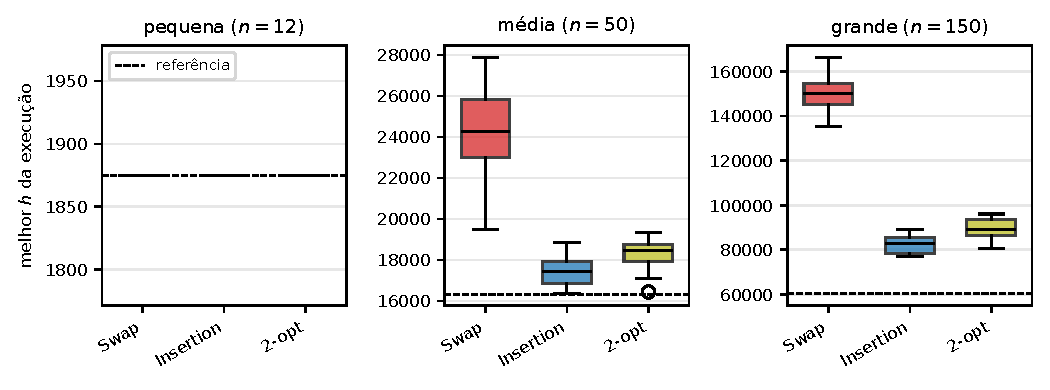
\includegraphics[width=\textwidth]{t2_vizinhancas}
  \caption{T2: melhor $h$ por execução da descida gulosa (\textit{first improvement}) em cada vizinhança.}
  \label{fig:t2}
\end{figure}

\begin{figure}[H]
  \centering
  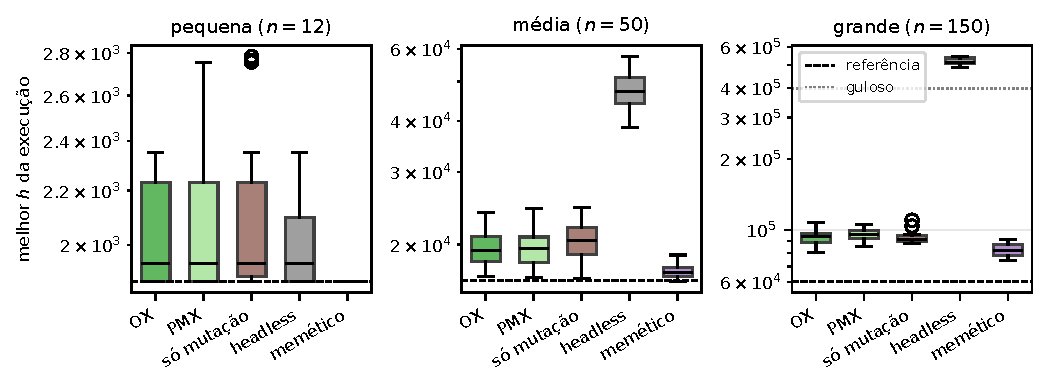
\includegraphics[width=\textwidth]{extra}
  \caption{Experimento extra: melhor $h$ por execução de cada variante do AG (escala logarítmica). A linha pontilhada é o guloso construtivo, desenhada quando cabe na escala.}
  \label{fig:extra}
\end{figure}

\section{Reprodução}
\label{ap:reproducao}

O código acompanha este relatório num arquivo separado, com um README que repete esta tabela.
Pré-requisitos: Python 3.12, \texttt{uv} e \texttt{make}; o primeiro comando é \texttt{make setup}.
Toda execução usa a semente $20\,261\,014 + 1\,000 \cdot i + r$, em que $i$ é o índice da instância e $r$ o da execução, e grava a semente no CSV.

\begin{table}[H]
  \centering\small
  \caption{Comando que gera cada resultado. As pastas de resultados levam a data da execução; as tabelas e figuras usam as pastas indicadas em \texttt{results/LATEST\_*}.}
  \label{tab:reproducao}
  \begin{tabular}{ll}
    \toprule
    Resultado & Comando \\
    \midrule
    Testes automáticos & \texttt{make test} \\
    T1 (saída da Seção~\ref{sec:t1}) & \texttt{make verify} \\
    T2 (execuções e tempo por movimento) & \texttt{make t2} \\
    Calibração do SA (Tabela~\ref{tab:sa-calibracao}) & \texttt{make calibrate} \\
    Exemplo do OX (Tabela~\ref{tab:ox}) & \texttt{make ox-demo} \\
    Pilotos de parâmetros do AG e do AG memético & \texttt{make ag-ajuste memetico-ajuste} \\
    T3 & \texttt{make experiments} \\
    Experimento extra & \texttt{make extra} \\
    Robustez (orçamento sem calibração e $2B$) & \texttt{make robustez} \\
    Tempos sem carga paralela & \texttt{make tempos} \\
    Todas as tabelas e figuras deste relatório & \texttt{make analysis} \\
    Este PDF & \texttt{make report} \\
    \bottomrule
  \end{tabular}
\end{table}
